\chapter{Anwendung von NLP in IT-Prozessen}
\label{cha:ApplicationsForNLPinProcesses}
\section{Allgemeines}

In diesem Kapitel wird erläutert, wie Natural Language Processing in ausgewählten IT-Prozessen Anwendung finden könnte, sowie die Verbesserung die dadurch erwartet wird. Es wird außerdem darauf eingegangen, welche technischen Limitierungen bzw. welche Probleme bei der Anwendung von Natural Language Processing noch entstehen, sowie ein Ausblick über die Machbarkeit gegeben.

Für die Analyse wird beschrieben, wie sich der Ablauf des Prozesses im Moment darstellt. Dazu wird der Ablauf mit Hilfe der \textit{BPMN}-Notation skizziert. Es wird erläutert wie die einzelnen Schritte im Detail abgearbeitet. Danach wird vermittelt, wie durch die Anwendung von \textit{NLP} eine Verbesserung erzielt werden kann. Dabei werden am Anfang eher einfachere Maßnahmen beschrieben, die leicht umzusetzen sind und keinen enormen Aufwand bedeuten, sowie einige eher komplexere Maßnahmen die teilweise weitere Voraussetzung, wie zum Beispiel, das Vorhandensein einer Wissensbasis, erfordern. Es wird ein Überblick gegeben, welche Schwierigkeiten sich ergeben und welche Vorteile durch die Anwendung von \textit{NLP} für die Prozessteilnehmer und den Prozess erzielt werden können.

\section{Das Beispielunternehmen}
Das Unternehmen \textit{XYZ Softwarehaus}, welches in den folgenden Abschnitten skizziert wird, ist ein klassisches Softwareentwicklungsunternehmen. Das XYZ Softwarehaus entwickelt und vertreibt dabei seine Software für die Planung von Meetings. Dabei wurden einige zentrale Geschäftsprozesse festgelegt, wovon die meisten klassische IT-Prozesse sind, die zwar mit Softwareunterstützung abgewickelt werden, jedoch keine Anwendung von \textit{NLP} stattfindet. Es wird im Folgenden beispielhaft auf folgende Geschäftsprozesse eingegangen, in denen \textit{NLP} möglicherweise eine Verbesserung bringen könnte:

\begin{enumerate}
	\item Supportprozess
	\item Neukundenprozess
\end{enumerate}

\section{Supportprozess}
Für die Abwicklung von Probleme oder allgemeinen Abfragen wurde im Unternehmen ein Supportprozess definiert. Dieser gibt vor, welche Schritte zu unternehmen sind und wie der Kunde schlussendlich zu einer Lösung kommt. In Abbildung \ref{fig:support-process} ist der Prozess in \textit{BPMN-Notation} dargestellt. 

\begin{figure}[ht]
	\centering
		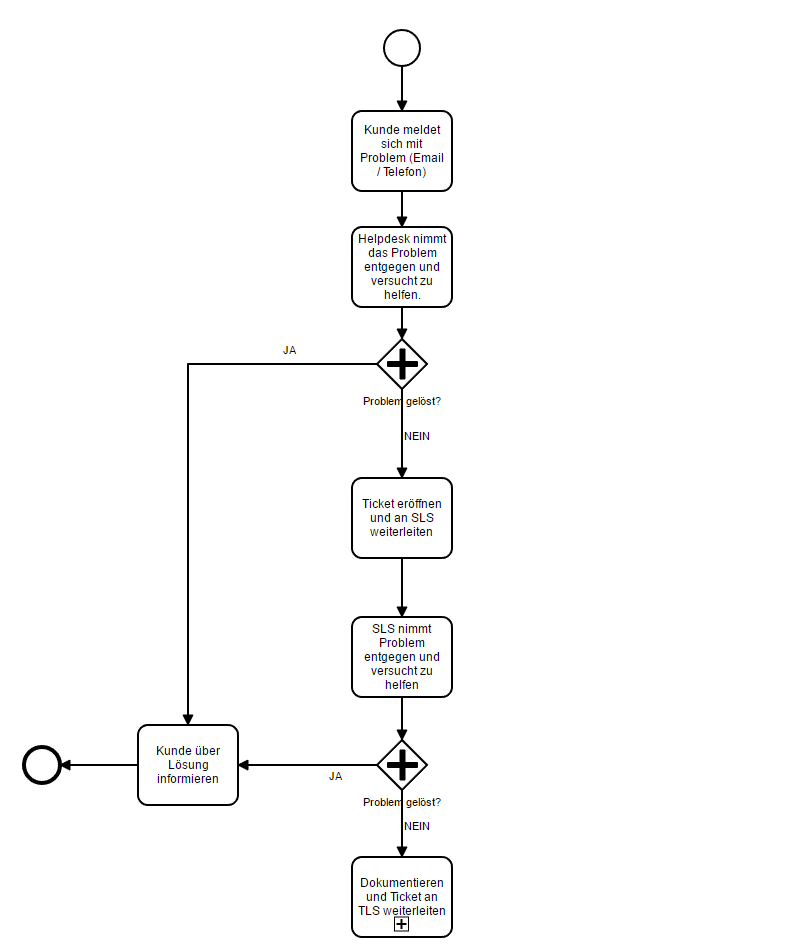
\includegraphics[width=0.80\textwidth]{images/support_process.PNG}
	\caption{Supportprozess des XYZ Softwarehauses}
	\label{fig:support-process}
\end{figure}

In dieser Abbildung sind die einzelnen Schritte des Prozesses dargestellt und es wird beschrieben wie diese abgearbeitet werden. Im Folgenden wird der Ablauf skizziert und geschildert, wie die einzelnen Schritte abgearbeitet werden und welche Ergebnisse geliefert werden.

\subsection{Ablauf}
Der erste Schritt des Prozesses ist die Anfrage eines Kunden über Email oder per Telefon. Dabei entstehen abhängig vom gewählten Medium unterschiedliche Daten. Diese stellen sich entweder in Form von Lautsprache, oder in Form von geschriebenem Text dar. Im Folgenden wird ausschließlich auf die Anfrage per Email eingegangen, da für die Anfrage per Telefon kein direkter Vorteil durch den Einsatz von \textit{NLP} erzielt werden kann, da hier vor allem auch der menschliche Kontakt eine wichtige Rolle spielt. %TODO EVENTUELL EINFÜGEN EINER STUDiE

Der Helpdesk nimmt die Anfragen des Kunden entgegen und versucht diese zu lösen. Dazu stehen dem Helpdesk mehrere Möglichkeiten zur Verfügung. In den meisten Fällen wird der Mitarbeiter am Helpdesk versuchen, Informationen zu dem gemeldeten Problem in der Wissensbasis zu finden. Dazu wird die Wissensbasis mit Schlagwörtern durchsucht, die das Anliegen des Kunden möglichst gut wiedergeben sollten. Kann keine Information aus der Wissenbasis gefunden werden kann versucht werden, das Problem ohne das vorhandene Wissen zu lösen. Falls eine Lösung auf einem anderen Weg gefunden werden kann, wird der Mitarbeiter die Informationen zur Lösung in der Wissensbasis hinzufügen und den Kunden über die Lösung des Problems informieren. Für jede Lösung wird dem Kunden zusätzlich ein Link zu dem Artikel mit der Lösung in der Wissenbasis übermittelt. Dies führt im Idealfall dazu, dass der Kunde in Zukunft ohne Hilfe des Helpdesks zu einer Lösung kommt.

Kann auf Grund der Komplexität des Problems im ersten Schritt vom Helpdesk keine Lösung gefunden werden, wird überprüft, ob bereits ein Ticket für dieses Problem geöffnet wurde. Möglicherweise ist das gemeldete Problem bereits bei anderen Kunden aufgetreten und daher auch schon im Ticketsystem vermerkt. Dieses manuelle auffinden der Tickets ist sehr häufig mit einigem an Zeitaufwand verbunden und häufig werden doppelt erstellte Tickets erst später entdeckt. Falls das Problem noch nicht in Form eines Tickets beschrieben wurde, wird ein Ticket erstellt, welches alle bereits im Helpdesk erhaltenen Informationen enthält und an den sogenannten \textit{Second Level Support (SLS)} weitergeleitet. Wenn im SLS eine Lösung gefunden werden kann, folgen die gleichen Schritte wie bei erfolgreicher Abarbeitung im Helpdesk: Der Kunde wird informiert und die Wissenbasis ergänzt. Zusätzlich wird dem Helpdesk eine Information gegeben, dass die Wissensbasis um die nötigen Informationen erweitert wurde, sodass bei zukünftigen Anfragen dieser Art eine Lösung möglicherweise schon beim Helpdesk gelöst werden kann.

Wenn das Problem auch im SLS nicht gelöst werden kann, geht es schließlich zum sogenannten \textit{Third Level Support(TLS)}. Dieser Teil des Prozesses ist in Abbildung \ref{fig:support-process} nur als Subprozess modelliert, da er sich sehr ähnlich gestaltet wie der Prozessschritt im SLS. Das Ergebnis dieses Prozessschrittes ist erneut, die Rückmeldung für den Kunden und die Erweiterung der Wissenbasis, sowie die Information des Helpdesks und des SLS über die Erweiterung.

Im Endeffekt sollte durch die kontinuierliche Erweiterung und Verbesserung der Wissenbasis ein System geschaffen werden, dass immer mehr Probleme direkt vom Kunden selbst gelöst werden können, oder bereits vom Helpdesk. Vor allem technische Probleme werden sehr häufig nur im SLS oder im TLS lösbar sein, da im Helpdesk schlichtweg keine Zeit für die Lösung dieser bleibt. 

\subsection{Verbesserung 1 - Kategorisierung der Anfrage}
Die erste Verbesserung die im Zuge des Supportprozesses vorgenommen werden kann ist eine Kategorisierung der Anfrage. Die meisten Email Programme und Mailserver bieten bereits eine grundlegende Kategorisierung über sogenannte Regeln an. Es kann zum Beispiel festgelegt werden, dass alle Emails die von einem bestimmten Absender kommen, in ein bestimmtes Unterverzeichnis verschoben werden können. In Abbildung \ref{fig:outlook-rules} ist ein Dialog für das Festlegen von Regeln in \textit{Microsoft Office 2016} dargestellt. Diese regelbasierte bietet bereits eine sehr einfache Möglichkeit der Vorsortierung der Emails, leider ist der Konfigurationsaufwand für das Erstellen dieser Regeln oft sehr groß. Die Regeln sind sehr strikt und können nur sehr einfache Bedingungen enthalten. Es ist z.B. nicht möglich, alle Emails von einer gemeinsamen Domain (microsoft.com) in ein Unterverzeichnis weiterzuleiten. Weiters gibt es keine Möglichkeiten die Mails auf den Inhalt zu prüfen und Regeln anzugeben, die abhängig vom Inhalt Mails Kategorisieren.

\begin{figure}[ht]
	\centering
		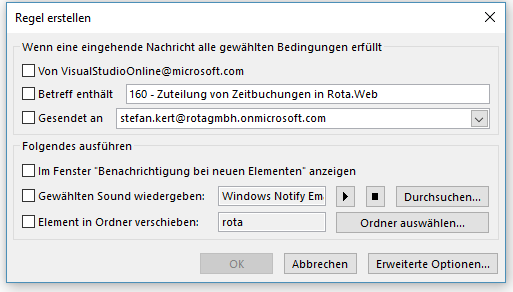
\includegraphics[width=0.80\textwidth]{images/outlook_rules.PNG}
	\caption{Dialog zum Festlegen von Regeln in MS Outlook}
	\label{fig:outlook-rules}
\end{figure}

Hier kann eine Anwendung von \textit{NLP} zum Beispiel dazu dienen, dass abhängig vom Inhalt der Mail Kategorien zugeordnet werden, oder komplexere Regeln für die Vorsortierung gewählt werden können. Mit Hilfe der \textit{Named Entity Recognition} können bereits Wörter ausgewählt werden die häufig vorkommen und abhängig von diesen eine Weiterleitung an spezielle Stellen eingerichtet werden. Ein Beispiel hierfür wäre folgendes Szenario:

Kunde A stellt eine Anfrage über die Möglichkeiten der Lizenzerweiterung. Die Email geht direkt in den sogenannten \textit{Office-Posteingang} der als gemeinsames Postfach für das Unternehmen verwendet wird. Dieser Posteingang wird vom Helpdesk verwaltet. Im Moment leitet der Helpdesk die Anfragen direkt an den Vertrieb weiter, da es sich um keine Supportanfragen handelt. 

Da Entscheidung über eine Weiterleitung an den Vertrieb auf dem Inhalt der Email basiert kann hier eine Anwendung von \textit{NLP} erfolgen. Der Text kann direkt beim Eingehen der Email vorab geprüft werden und sobald bestimmte Kriterien erfüllt werden, erfolgt eine automatische Weiterleitung an den \textit{Vertrieb}. Diese Kriterien reichen von einfachen Regeln, wie dem Inhalt von Schlagwörtern, bis zu komplexeren Kriterien wie der beschriebenen  \textit{Named Entity Recognition} die über die Anwendung einer \textit{Taxonomie} auch eine Klassifizierung von Wörter ermöglicht.

\subsubsection{Vorteile}
Für diese Verbesserung ergeben sich folgende Vorteile:

\begin{itemize}
	\item Bessere Vorverarbeitung von Emails
	\item Automatisches Zuordnen zu den richten Stellen für Emails
	\item Komplexere Regeln möglich
\end{itemize}

\subsubsection{Machbarkeit}
Wie bereits eingangs erwähnt sind diese Maßnahmen relativ leicht umzusetzen. Das Zuordnen von Stichwörtern entspricht nicht direkt dem \textit{NLP} sondern sind eher fix definierte Regeln und es gibt bereits Tools die dies ermöglichen. Das Anwenden einer \textit{Taxonomie} für die Klassifizierung und Zuordnung erfordert eine Integration in das System. Dies könnte beispielsweise über Plugins realisiert werden. Vor allem im englischsprachigem Bereich gibt es sehr umfangreiche \textit{Taxonomien} die auch eine sehr komplexe Zuordnung erlauben. Für die Anwendung von \textit{NER} gilt sehr ähnliches wie für die \textit{Taxonomie}. Auch ihre Anwendung erfordert eine tiefere Integration ins System. Auch hier hat man mit englischsprachigem Inhalt mehr Möglichkeiten als für deutsche Texte. Grundsätzlich lässt sich für diese Verbesserung zusammenfassend sagen, dass ein Einstieg über die Zuordnung über Schlagwörter bereits einen Vorteil und eine Prozessoptimierung bringen würde, da diese Aufgabe, die vom Helpdesk nach vorgegeben Regeln abgearbeitet wird, über diese Zuordnung nach Schlagwörtern auch automatisiert passieren kann. Im ersten Schritt wäre es also möglich, diese Weiterleitung auf Grund von Schlagwörtern mit einer einfachen Liste zu verwalten, welche im Prinzip \textit{m:1} Beziehungen darstellt, die ein Mapping von Wörtern zu Emails repräsentieren. Die Email wird schließlich der Email zugeordnet, bei der die meisten Regeln erfüllt sind. 

\subsection{Verbesserung 2 - Hinzufügen von Informationen aus der Wissensbasis}
Ein sich im Prozess immer wiederholender Schritt ist die kontinuierliche Erweiterung der Wissenbasis, sowie die Verwendung der darin enthaltenen Informationen. Hier wird im Moment durch manuelles Durchsuchen dieser Wissenbasis versucht Informationen zu erhalten. Dies ist mit sehr viel Aufwand verbunden, da der Helpdeskmitarbeiter die Schlagwörter oder Inhalte die in der Email enthalten sind einzeln in der Wissenbasis eingeben muss und schließlich aus den Ergebnissen eine Antwort zusammenfassen muss. Dies ist häufig mit sehr viel Zeit und Aufwand verbunden und liefert aber häufig sehr gute Ergebnisse die genau auf das Problem des Kunden zugeschnitten sind. 

Um die Effizienz dieser Suche zu Steigern kann mit Hilfe von \textit{NLP} nach einer Vorverbarbeitung und Kategorisierung der Anfrage, ein automatisches Durchsuchen der Wissenbasis erfolgen. Dabei wird die Wissenbasis gleich wie beim manuellen Durchsuchen nach bestimmten Schlagwörtern oder Szenarien durchsucht, und die Ergebnisse ausgewertet. Wie bei vielen textbasierenden Suchmaschinen oder Algorithmen ist es auch hier möglich ein Ranking nach der Relevanz der einzelnen gefunden Informationen im Bezug auf die Suche anzugeben. Das Ergebnis ist eine Liste an Artikeln die nach der Relevanz sortiert sind.

Der Mitarbeiter des Helpdesks hat nun die Möglichkeit, dem Kunden einen Artikel aus der erhaltenen Liste zurückzusenden, wodurch noch eine weitere manuelle Überprüfung der erhaltenen Informationen auf Korrektheit möglich ist. 

Hier wäre es möglich, durch die Rückgabe der Auswahl des Artikels durch den Kundenbetreuer, das Model für die Auswahl der Artikel weiter zu trainieren. Wenn beispielsweise keiner der Artikel zu der gestellten Anfrage passt, kann eine manuelle Suche durch den Helpdeskmitarbeiter erfolgen. Wenn bei dieser manuellen Suche ein Artikel gefunden werden konnte, wird mit dieser Information das Model trainiert, sodass in Zukunft ein besseres Ergebnis erzielt werden kann.

Dieses Trainieren des Models kann schließlich auch für die manuelle Suche in der Wissenbasis helfen, von dem schlussendlich auch Kunden und Helpdeskmitarbeiter profitieren, da die Ergebnisse, die zu Anfragen gefunden werden, durch das Trainieren des Models immer genauer werden.

Am Ende sollte der Helpdeskmitarbeiter die Möglichkeithaben, nach der manuellen Auswahl des Artikels, eine Email generieren zu lassen, die alle nötigen Informationen wie Links zum Artikel in der Wissenbasis, oder auch den Artikel im PDF Format als Anhang mitzusenden. 

Ein weiterer möglicher Schritt wäre, die Rückmeldung des Kunden, ob der Artikel für die aufgetretene Problematik relevant ist, auch wieder ins System zurückfließen zu lassen und so das Model weiter trainiert wird. Hier, wie auch bei der Auswahl durch den Helpdeskmitarbeiter, besteht natürlich die Gefahr, dass eine falsche Auswahl getroffen wird und auf Grund dessen eine falsche Information ins Model gelangt. Um diese Problematik so gering wie möglich zu halten, erfordert es vor allem am Anfang, wenn das Model noch nicht sehr ausgeprägt trainiert ist, eine hohe Genauigkeit am Helpdesk.

\subsubsection{Vorteile}
Für diese Verbesserung ergeben sich folgende Vorteile:

\begin{itemize}
	\item Schnelles und automatisches Erhalten von Informationen aus der Wissenbasis
	\item Geringer manueller Aufwand für Helpdesk
	\item Manuelle Suche wird durch Trainieren des Models verbessert
\end{itemize}

\subsubsection{Machbarkeit}
Wie auch schon bei Verbesserung 1 erfordert Verbesserung 2 zahlreiche Maßnahmen die im Vorhinein getroffen werden müssen. Wenn für das Unternehmen keine Wissenbasis vorhanden ist, oder diese nur unzureichend befüllt ist, wird diese Verbesserung keinen Vorteil für das Unternehmen bringe, da entweder gar keine oder nur schlechte Ergebnisse geliefert werden. Wichtig ist vor allem der manuelle Input. Das Model für die Suche der Daten sollte im Idealfall laufend trainiert werden, sodass die Ergebnisse im Laufe der Zeit immer besser werden. Dies bedäutet vor allem am Anfang einen erhöhten manuellen Aufwand. Häufig gibt es bereits eine Auswertung wie hilfreich gewisse Informationen aus der Wissenbasis sind, dies kann natürlich für das Reihen der Informationen nach Relevanz verwendet werden. Auch hier gilt wieder, dass eine einfache Implementierung bereits einige Vorteile bringt, auch wenn die Zeitersparnis nur daraus besteht, dass der Mitarbeiter oder die Mitarbeiterin nicht die Wissensbasis durchsuchen muss, oder dies erst tun muss, wenn die gelieferten Ergebnisse unzufriedenstellend sind. 

\subsection{Verbesserung 3 - Erkennen von duplizierten Tickets}
Wenn das Problem von einem Mitarbeiter oder Mitarbeiterin des Helpdesk nicht gelöst werden kann, wird ein sogenanntes Ticket erstellt. Dieses Ticket enthält Informationen über das Problem, den Kunden oder die Kundin, wo das Problem aufgetreten ist und weitere Metainformationen wie, Betriebssystem, Version der Applikation oder auch ob das Problem nur zu einer bestimmten Uhrzeit auftritt. Vor der Erstellung dieses Tickets, wird das Ticketsystem noch auf ähnliche Probleme durchsucht. Häufig ergibt diese Suche, dass einige Probleme bereits gemeldet wurden. Ist dies der Fall wird das neue Ticket mit dem alten Ticket verküpft, dass beide gemeinsam gelöst werden können. Dieser Schritt erfordert erneut eine manuelle Suche die durch einen Mitarbeiter oder eine Mitarbeiterin des Helpdesks erfolgen muss. Hier könnte eine Verbesserung durch die Anwendung von \textit{NLP} dadurch erreicht werden, dass sobald ein Ticket erstellt wird, die Wissensbasis automatisch nach ähnlichen oder gleichen Tickets durchsucht wird. Es sollten also Duplikate von Tickets erkannt werden und dem Mitarbeiter oder der Mitarbeiterin eine Rückmeldung gegeben werden, dass dieses oder ein ähnliches Ticket bereits erstellt wurde. Auch hier erfordert es wieder eine manuelle Eingabe des Mitarbeiters oder der Mitarbeiterin. Es wird bei dieser Zuordnung überprüft, ob die ermittelten Ergebnisse wirklich übereinstimmen. Ist dies der Fall, wird das Ticket zugeordnet.

\subsubsection{Vorteile}
Für diese Verbesserung ergeben sich folgende Vorteile:

\begin{itemize}
	\item Schnelles und automatisches Auffinden von duplizierten Tickets
	\item Weniger Tickets kommen zum SLS oder zum TLS, da duplizierte Tickets bereits zuvor zusammengefasst werden
\end{itemize}

\subsubsection{Machbarkeit}
Die Funktionalität, welche für diese Verbesserung benötigt wird, ist wie auch bei der Wissensbasis eine einfache textbasierte Suche. Die vorhandenen Tickets werden mit dem neuen Ticket verglichen und die Ähnlichkeit der beiden Tickets ist ausschlaggebend für die Reihung der Ergebnisse. Dies könnte beispielsweise über ein Plugin für das Ticketsystem gelöst werden.

\section{Neukundenprozess}
Die Anfrage und die Abarbeitung der Anfragen von Neukunden, stellt einen weiteren wichtigen Geschäftsprozess im Unternehmen dar.  In Abbildung \ref{fig:neukunde-process} ist der Prozess in \textit{BPMN-Notation} dargestellt. 

\begin{figure}[ht]
	\centering
		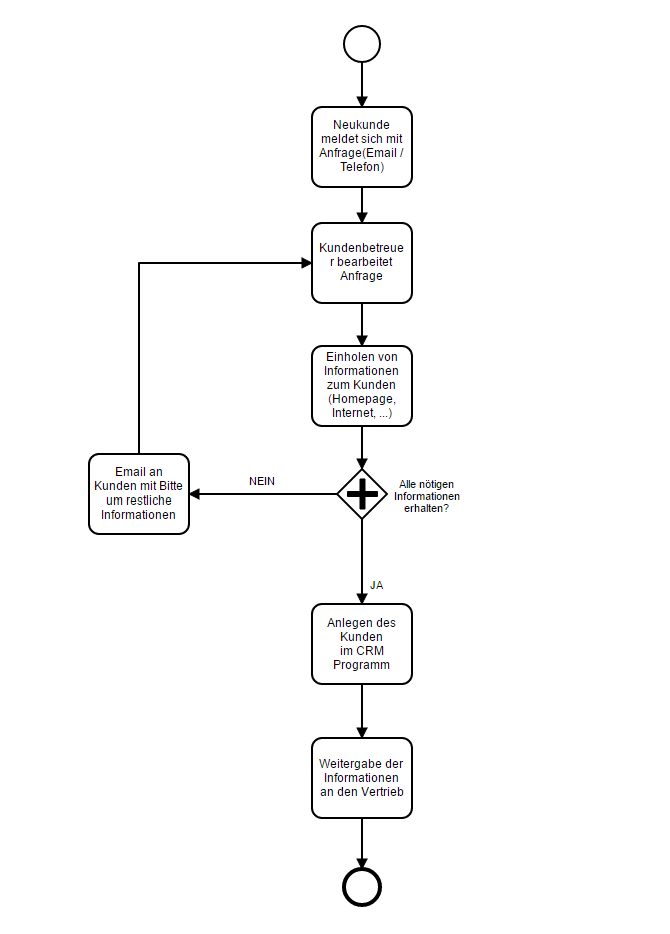
\includegraphics[width=0.80\textwidth]{images/neukunde_prozess.PNG}
	\caption{Neukundenprozess des XYZ Softwarehauses}
	\label{fig:neukunde-process}
\end{figure}

\subsection{Ablauf}
Gleich wie beim Supportprozess startet der Prozess mit der Anfrage eines Kunden. Dabei ist der Unterschied zum Supportprozess, dass diese Anfrage von jemanden kommt, der im CRM-System noch nicht vorhanden ist und für den noch keine Daten hinterlegt sind. Nach Erhalt der Anfrage, per Telefon oder per Email, wird diese von einem Kundenbetreuer bearbeitet. Dabei wird mit den in der Anfrage enthaltenen Informationen nach weiteren Informationen gesucht. Wenn die Anfrage beispielsweise einen Link zur Homepage enthält, wird diese Homepage konsultiert und die darin enthaltenen Informationen wie Standort, Branche oder auch die Anzahl der Mitarbeiter dokumentiert. Weiters wird mit Hilfe einer Onlinesuche noch nach weiteren Informationen gesucht, die für den Verkaufsprozess von Bedeutung sind. Falls noch Fragen offen sind, oder Informationen nicht oder nur teilweise erhalten werden konnten, wird dem Kunden eine Anfrage mit der Bitte um Zusendung der restlichen Informationen zugesendet. Die Rückmeldung auf diese Anfrage wird erneut vom Kundenbetreuer bearbeitet und falls alle wichtigen Informationen vorhanden sind, wird er Kunde im CRM angelegt und die Information an den Vertrieb weitergegeben. Dies ist Zugleich der Auslöser für den Verkaufsprozess.

\subsection{Verbesserung 1 - Automatisches Auslesen der Informationen aus der Email}
Eine erste Möglichkeit für eine Verbesserung ist das automatische Auslesen der bereits in der Email enthaltenen Informationen. Häufig werden für Neukundenanfragen Formulare verwendet. Diese ermöglicht das automatische Auslesen ungemein, da es immer nach einem fixen Muster vorgenommen werden kann. Durch die Anwendung von \textit{NLP} wird es auch möglich, Informationen, welche im Fließtext vorhanden sind auszulesen. Durch die Anwendung der \textit{Named Entity Recognition} können bereits einige Informationen wie, Personen, Firmenname, Adressen etc. ausgelesen werden. Das Ergebnis ist eine Liste, die der Kundenbetreuer oder die Kundenbetreuerin überprüft, verbessert und schließlich im System hinterlegt. 


\subsubsection{Vorteile}
Für diese Verbesserung ergeben sich folgende Vorteile:

\begin{itemize}
	\item Automatisches Auslesen der Informationen aus der Email
\end{itemize}

\subsubsection{Machbarkeit}
Diese Verbesserung stellt sich als eher schwierig dar, da vor allem durch Rechtschreibfehler oder syntaktische Fehler im Text eine \textit{Named Entity Recognition} nicht die gewünschten Ergebnisse liefern wird. Meist ist es schneller, die erhaltenen Informationen durch einen Mitarbeiter oder eine Mitarbeiterin der Kundenbetreuungg manuell zu verarbeiten. Vorteile bringt diese Verbesserung nur bei sehr lange Emails, die sehr viele Informationen enthalten, oder auch bei einer sehr hohen Anzahl an Anfragen, dass bereits eine Vorverarbeitung dieser erfolgen kann. Bei kurzen Emails, oder wenn nur gelegentlich Anfragen kommen, ist der Aufwand für die Implementierung und der Aufwand für die manuelle Fehlerkorrektur nicht gerechtfertigt.


\subsection{Verbesserung 2 - Sammeln von Informationen}
In einem Schritt des Neukundenprozesses wird vom Kundenbetreuer oder der Kundenbetreuerin versucht, weitere Informationen über den Kunden im Internet zu finden. Meist wird dabei nach einem fixen Muster vorgegangen:

\begin{enumerate}
	\item Durchführen einer Suche im Internet nach dem Neukunden (evtl. ist die Webseite auch in der Anfrage enthalten)
	\item Durchsuchen der Webseite des Kunden nach relevanten Informationen
	\item Aufrufen des Impressums und notieren der darin enthaltenen Information
	\item Informationen notieren und später im CRM hinterlegen.
\end{enumerate}

Diese Schritte wiederholen sich prinzipiell bei jedem Neukunden. Die Anwendung von \textit{NLP} könnte hier auf zwei verschiedene Arten angestoßen werden:

\subsubsection{Automatisch}
Bei Erhalt einer Anfrage eines Neukunden wird die Anfrag automatisch nach Informationen zum Kunden durchsucht. Links die in der Email enthalten sind werden aufgerufen und überprüft, ob die Webseite weitere Informationen für den Kunden enthält. Dafür ist auch eine Überprüfung notwendig, ob die Webseite überhaupt dem Kunden zuzuordnen ist oder ob sich der Link aus einem anderen Grund in der Anfrage befunden hat. Ist keine Webseite und kein Link in der Anfrage enthalten wird mit Hilfe einer Suchmaschine nach dem Kunden gesucht. Hierfür werden die in der Anfrage enthaltenen Informationen verwendet. 

\subsubsection{Manuell}
Wenn die Anfrage keine Webseite für den Kunden enthält und auch keine Informationen zu einer erfolgreichen Suche führen, muss manuell eingegriffen werden. Der Kundenbetreuer oder die Kundenbetreuerin hat dann die Möglichkeit, die Verarbeitung der Webseitendaten manuell anzustoßen. Eine Möglichkeit zum Erhalt der nötigen Informationen wäre zum Beispiel eine Rückfrage beim Kunden. 

Nachdem die Verarbeitung angestoßen wurde und die Webseite vom Algorithmus durchsucht wurde wird im Idealfall eine Liste mit zusätzlichen Informationen zum Kunden ausgegeben. Diese Liste wird wiederum von einem Kundenbetreuer oder Kundenbetreuerin überprüft und eventuell erweitert oder ausgebessert. Die erhaltenen Informationen werden schließlich im CRM hinterlegt.

\subsubsection{Vorteile}
Für diese Verbesserung ergeben sich folgende Vorteile:

\begin{itemize}
	\item Automatisches Sammeln weiterer Informationen aus dem Internet 
	\item Umfangreichere Informationen zum Kunden
\end{itemize}

\subsubsection{Machbarkeit}
Wie auch schon beim automatischen Verarbeiten der Informationen, die in der Anfrage enthalten sind, erfordert die Verarbeitung der Daten auf der Webseite manuelle Arbeit. Die Überprüfung der Ermittelten Daten auf Korrektheit ist zwangsläufig notwendig, da viele Faktoren das automatische Auslesen der richtigen Daten schwierig gestalten. Ein Problem stellen falsch gepflegte Daten auf der Webseite dar, die durch einen Kundenbetreuer oder eine Kundenbetreuerin erkannt werden können, durch eine Verarbeitung mit Hilfe von \textit{NLP} aber nur sehr selten. Grundsätzlich wäre eine Anwendung der automatischen Informationsbeschaffung im Internet aber hilfreich, da dem Kundenbetreuer oder der Kundenbetreuerin sehr schnell viele Informationen zum Unternehmen zur Verfügung stehen die ausgewertet und verarbeitet werden können.
